Obviously, all we have faced the cases of crucial over-engineering during the implementation of some
software product.
For the programmer, it is a vital point to follow two separated, but closely related software development principles,
such that KISS [\cite{alwin2016kiss}], and YAGNI [\cite{da2018evolution}].
As the main topic of our thesis is to implement Instant Messaging System following the security and privacy aspects.
We consider to following above-mentioned development principles KISS and YAGNI and approach
a well-known N-tier application Monolithic architecture [\cite{bucchiarone2018monolithic}], which provides a model by which developers can
create flexible and reusable applications.
By segregating an application into tiers, developers acquire the option of modifying or adding a specific layer,
instead of reworking the entire application.
A three-tier architecture is typically composed of a presentation tier, a logic tier, and a data tier.
One would suggest to use nowadays popular Microservices Architecture, thinking about scalability [\cite{brataas2004exploring}],
an ability of the system to handle large numbers of users distributed over geographically large areas without
notably affecting the overall performance of the system.
However, the effect of Microservices is being felt only for quite large and complex systems,
not the case of our yet simple application.
Following plot demonstrates this relation

\begin{figure}[H]
    \centering
    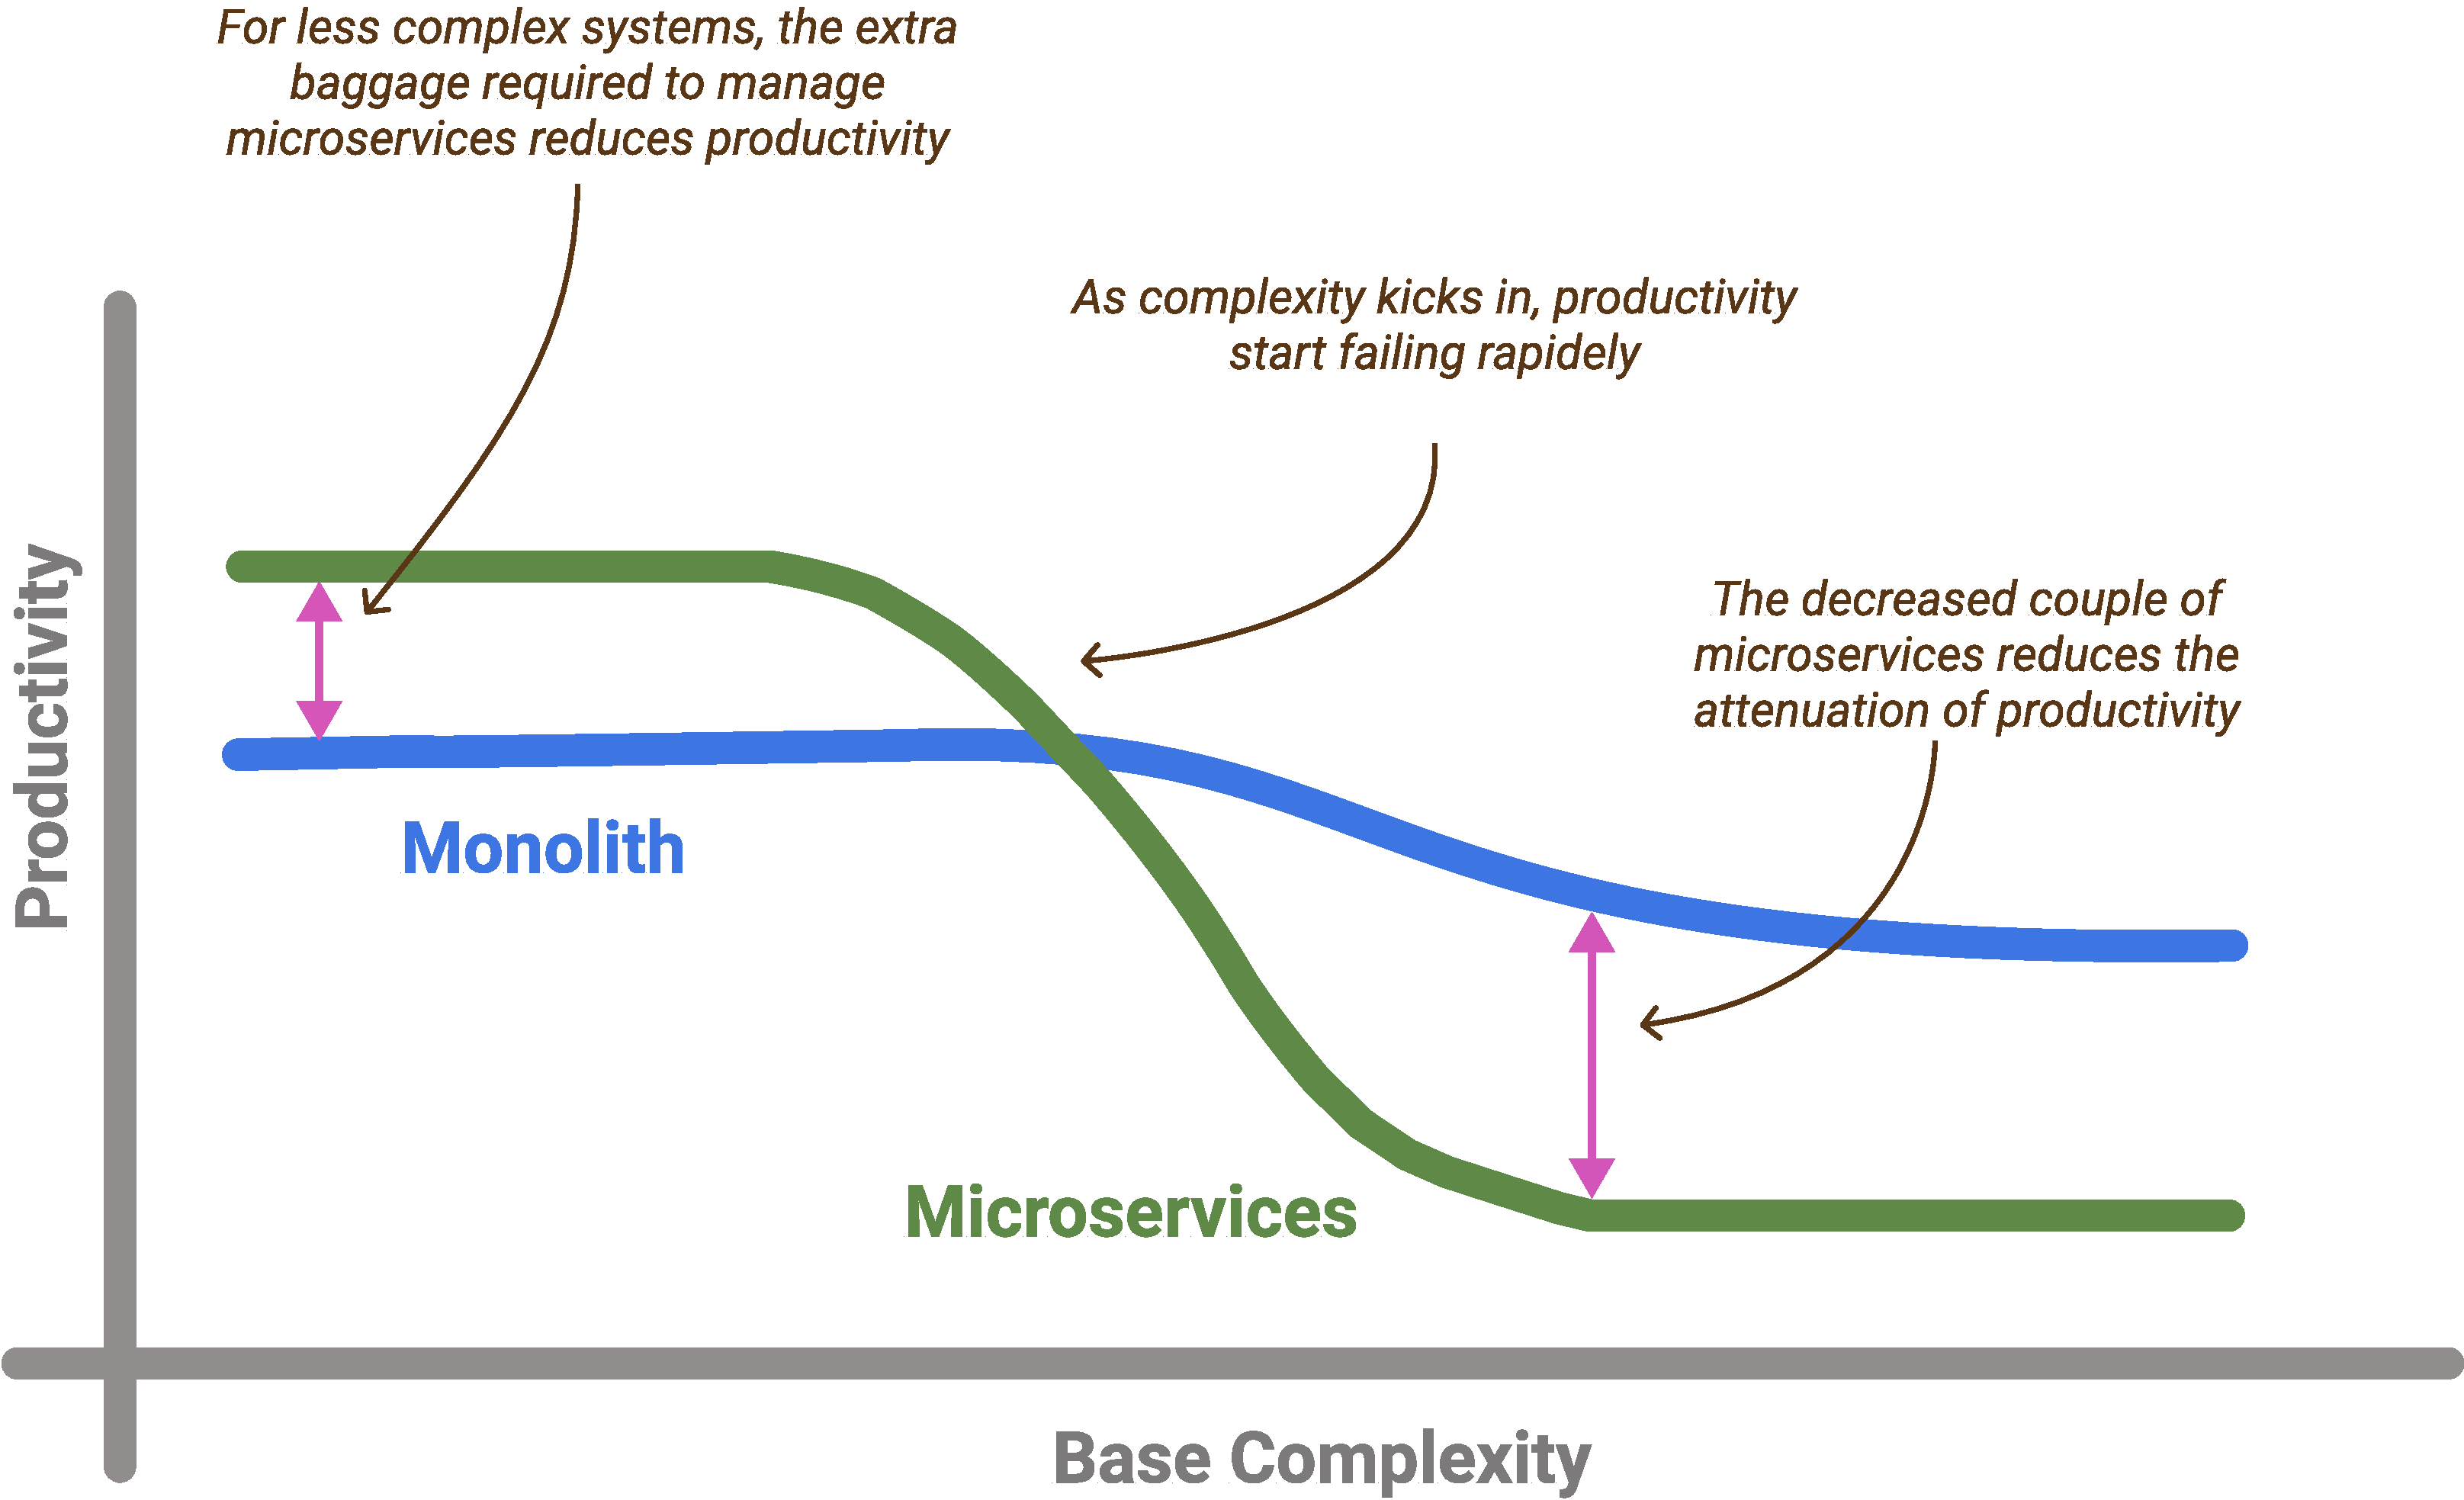
\includegraphics[width=1\textwidth]{Pictures/Monolith_vs_Microservice.pdf}
    \caption{Relation between system complexity and architectures.
    Source: \href{https://martinfowler.com/bliki/MicroservicePremium.html}{Martin Fowler.}}
    \label{fig:monolith_vs_microservice}
\end{figure}

In a logical multilayer architecture for an information system with an object-oriented design, the following four are the most common:

\begin{itemize} % source: https://en.wikipedia.org/wiki/Multitier_architecture#cite_note-5
    \item \textbf{Presentation Layer.} UI layer, view layer, presentation tier in multitier architecture.
    \item \textbf{Application Logic.} Service layer [\cite{ji2009intelligent, swetina2014toward}]
    or GRASP Controller Layer [\cite{okada2006vision}].
    \item \textbf{Business Logic.} Business logic layer, domain logic layer.
    \item \textbf{Data Access Layer.} Persistence layer, logging, networking, and other services which are required
    to support a particular business layer.
\end{itemize}

\begin{figure}[H]
    \centering
    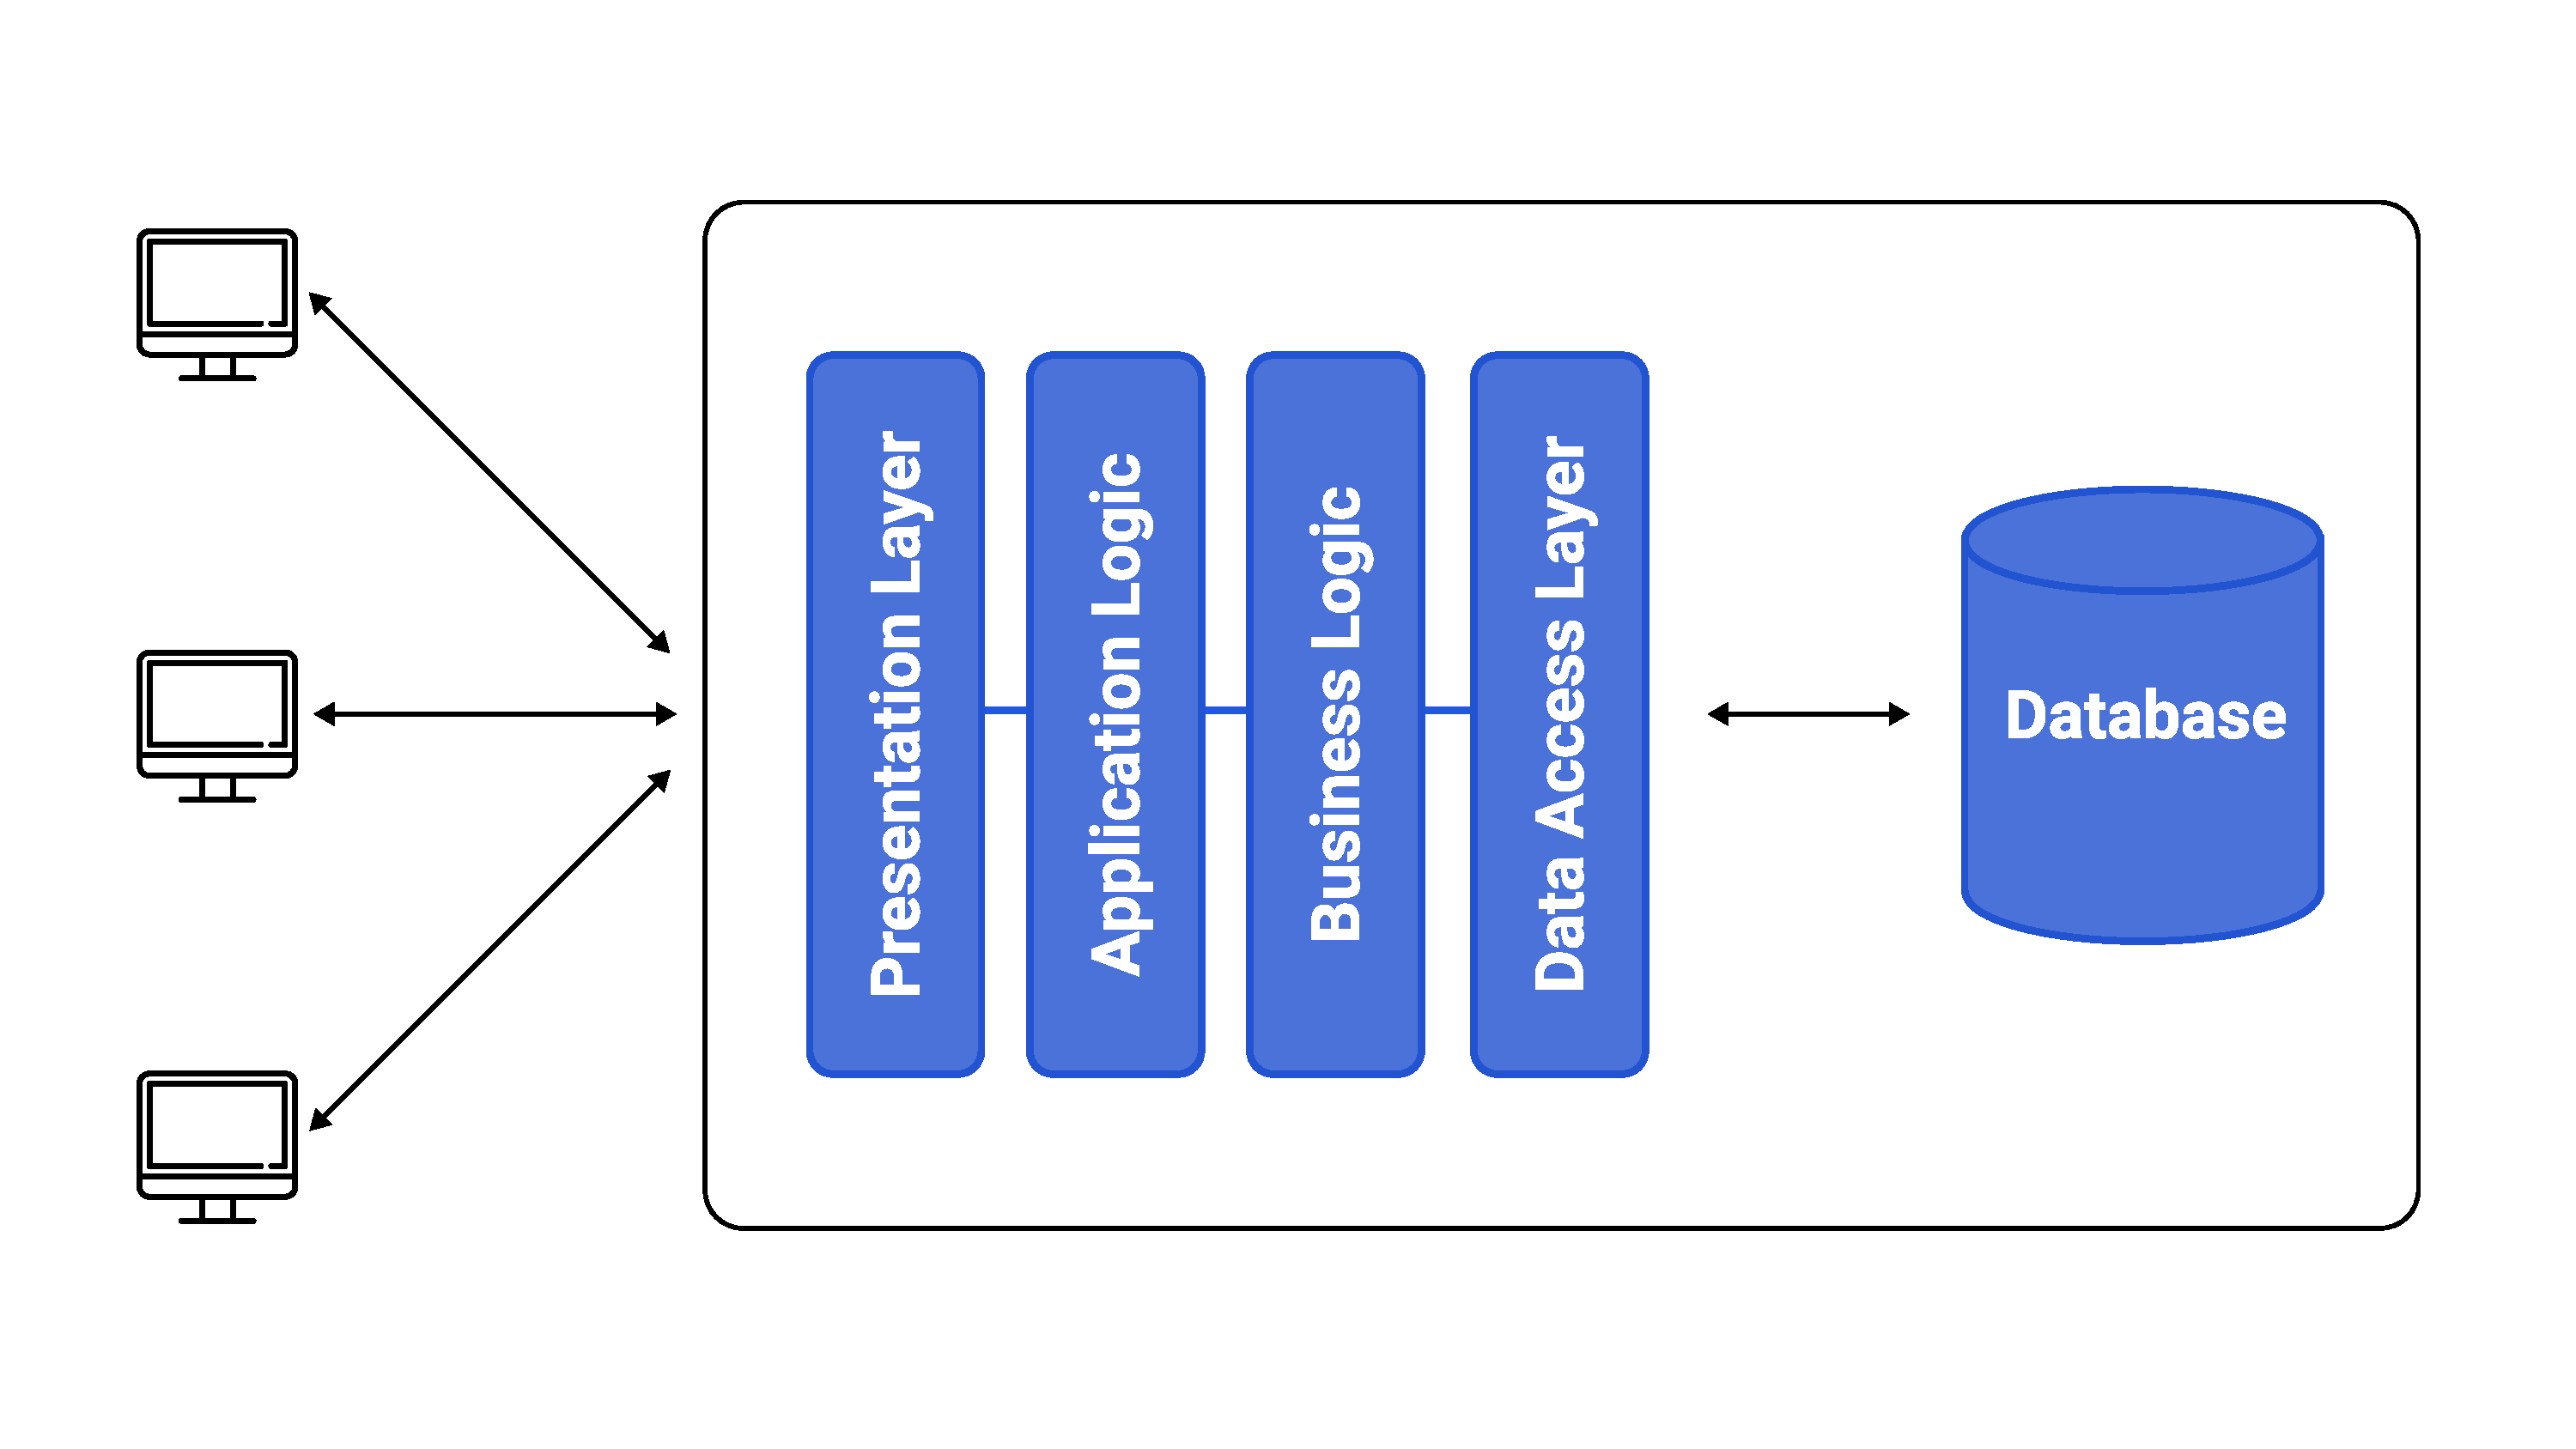
\includegraphics[width=1\textwidth]{Pictures/Monolith_architecture.pdf}
    \caption{Monolithic architecture diagram.}\label{fig:figure2}
\end{figure}

The book Domain Driven Design [\cite{solvberg2010domain}] describes some common uses for the above four layers, although its primary focus is the
domain layer.
If the application architecture has no explicit distinction between the business layer and the presentation layer,
then a traditional client-server model has been implemented.
The presentation layer is considered part of the business layer.
The more usual convention is that the application layer is considered a sublayer of the business layer,
typically encapsulating the API definition surfacing the supported business functionality.
The application/business layers can, in fact, be further subdivided to emphasize additional sub-layers of distinct
responsibility.
For example, if the model–view–presenter pattern is used, the presenter sublayer might be used as an additional layer
between the user interface layer and the business/application layer, as represented by the model sublayer.
Some also identify a separate layer called the business infrastructure layer, located between the business layer
and the infrastructure layer.
It's also sometimes called the \textit{low-level business layer} or the \textit{business services layer}.
The infrastructure layer can be partitioned into different levels, high-level or low-level technical services [\cite{dennis2018mcapl}].
Developers often focus on the persistence capabilities of the infrastructure layer and therefore only
talk about the persistence layer or the data access layer instead of an infrastructure layer or technical services layer.
In other words, the other kind of technical services are not always explicitly thought of as part of any particular layer.
A layer is on top of another, because it depends on it.
Every layer can exist without the layers above it, and requires the layers below it to function.
Another common view is that layers do not always strictly depend on only the adjacent layer below.
For example, in a relaxed layered system, a layer can also depend on all the layers below it [\cite{anon2014building}].
Relaxed layered system may be considered as opposed to a strict layered system.

\subsection{Monolith Architecture: Cons and Props}\label{subsec:monolith-architecture:-cons-and-props}

A monolith is built as a large system with a single code base and deployed as a single unit, usually behind a load balancer.
It typically consists of four major components: a user interface, business logic, a data interface and a database.
Monoliths offer several advantages, particularly when it comes to operational overhead requirements.
Here are some of those basic benefits:

\begin{itemize}
    \item \textbf{Simplicity.} Monolithic architectures are simple to build, test and deploy.
    These apps can scale horizontally, in one direction, by running several copies of the application behind a load balancer.
    Cross-cutting concerns: With a single codebase, monolithic apps can easily handle cross-cutting concerns, such as logging,
    configuration management and performance monitoring.
    Another advantage associated with the simplicity of monolithic apps is easier deployment.
    When it comes to monolithic applications, you do not have to handle many deployments – just one file or directory.
    \item \textbf{Performance.} Components in a monolith typically share memory which is faster than service-to-service
    communications using IPC [\cite{proctor1999linux}] or other mechanisms.
    \item \textbf{Easier debugging and testing.}
    In contrast to the microservices architecture, monolithic applications are much easier to debug and test.
    Since a monolithic app is a single indivisible unit, you can run end-to-end testing much faster.
    \item \textbf{Easier development.} As long as the monolithic approach is a standard way of building applications,
    any engineering team has the right knowledge and capabilities to develop a monolithic application.
\end{itemize}
But one major drawback of monolithic architectures is tight coupling.
Over time, monolithic components become tightly coupled and entangled.
This coupling effects management, scalability and continuous deployment.
Other cons that stem from tight coupling include:
\begin{itemize}
    \item \textbf{Understanding.} When a monolithic application scales up, it becomes too complicated to understand.
    Also, a complex system of code within one application is hard to manage.
    \item \textbf{Reliability.} An error in any of the modules in the application can bring the entire application down.
    \item \textbf{Updates.} Due to a single large codebase and tight coupling, the entire application would have to deploy
    for each update.
    \item \textbf{Technology stack.} A monolithic application must use the same technology stack throughout.
    Changes to the technology stack are expensive, both in terms of the time and cost involved.
    \item \textbf{Scalability.} You cannot scale components independently, only the whole application.
\end{itemize}

\subsection{Decoupling Monolith using CQRS}\label{subsec:decoupling-monolith-using-cqrs}
\begin{figure}[H]
    \centering
    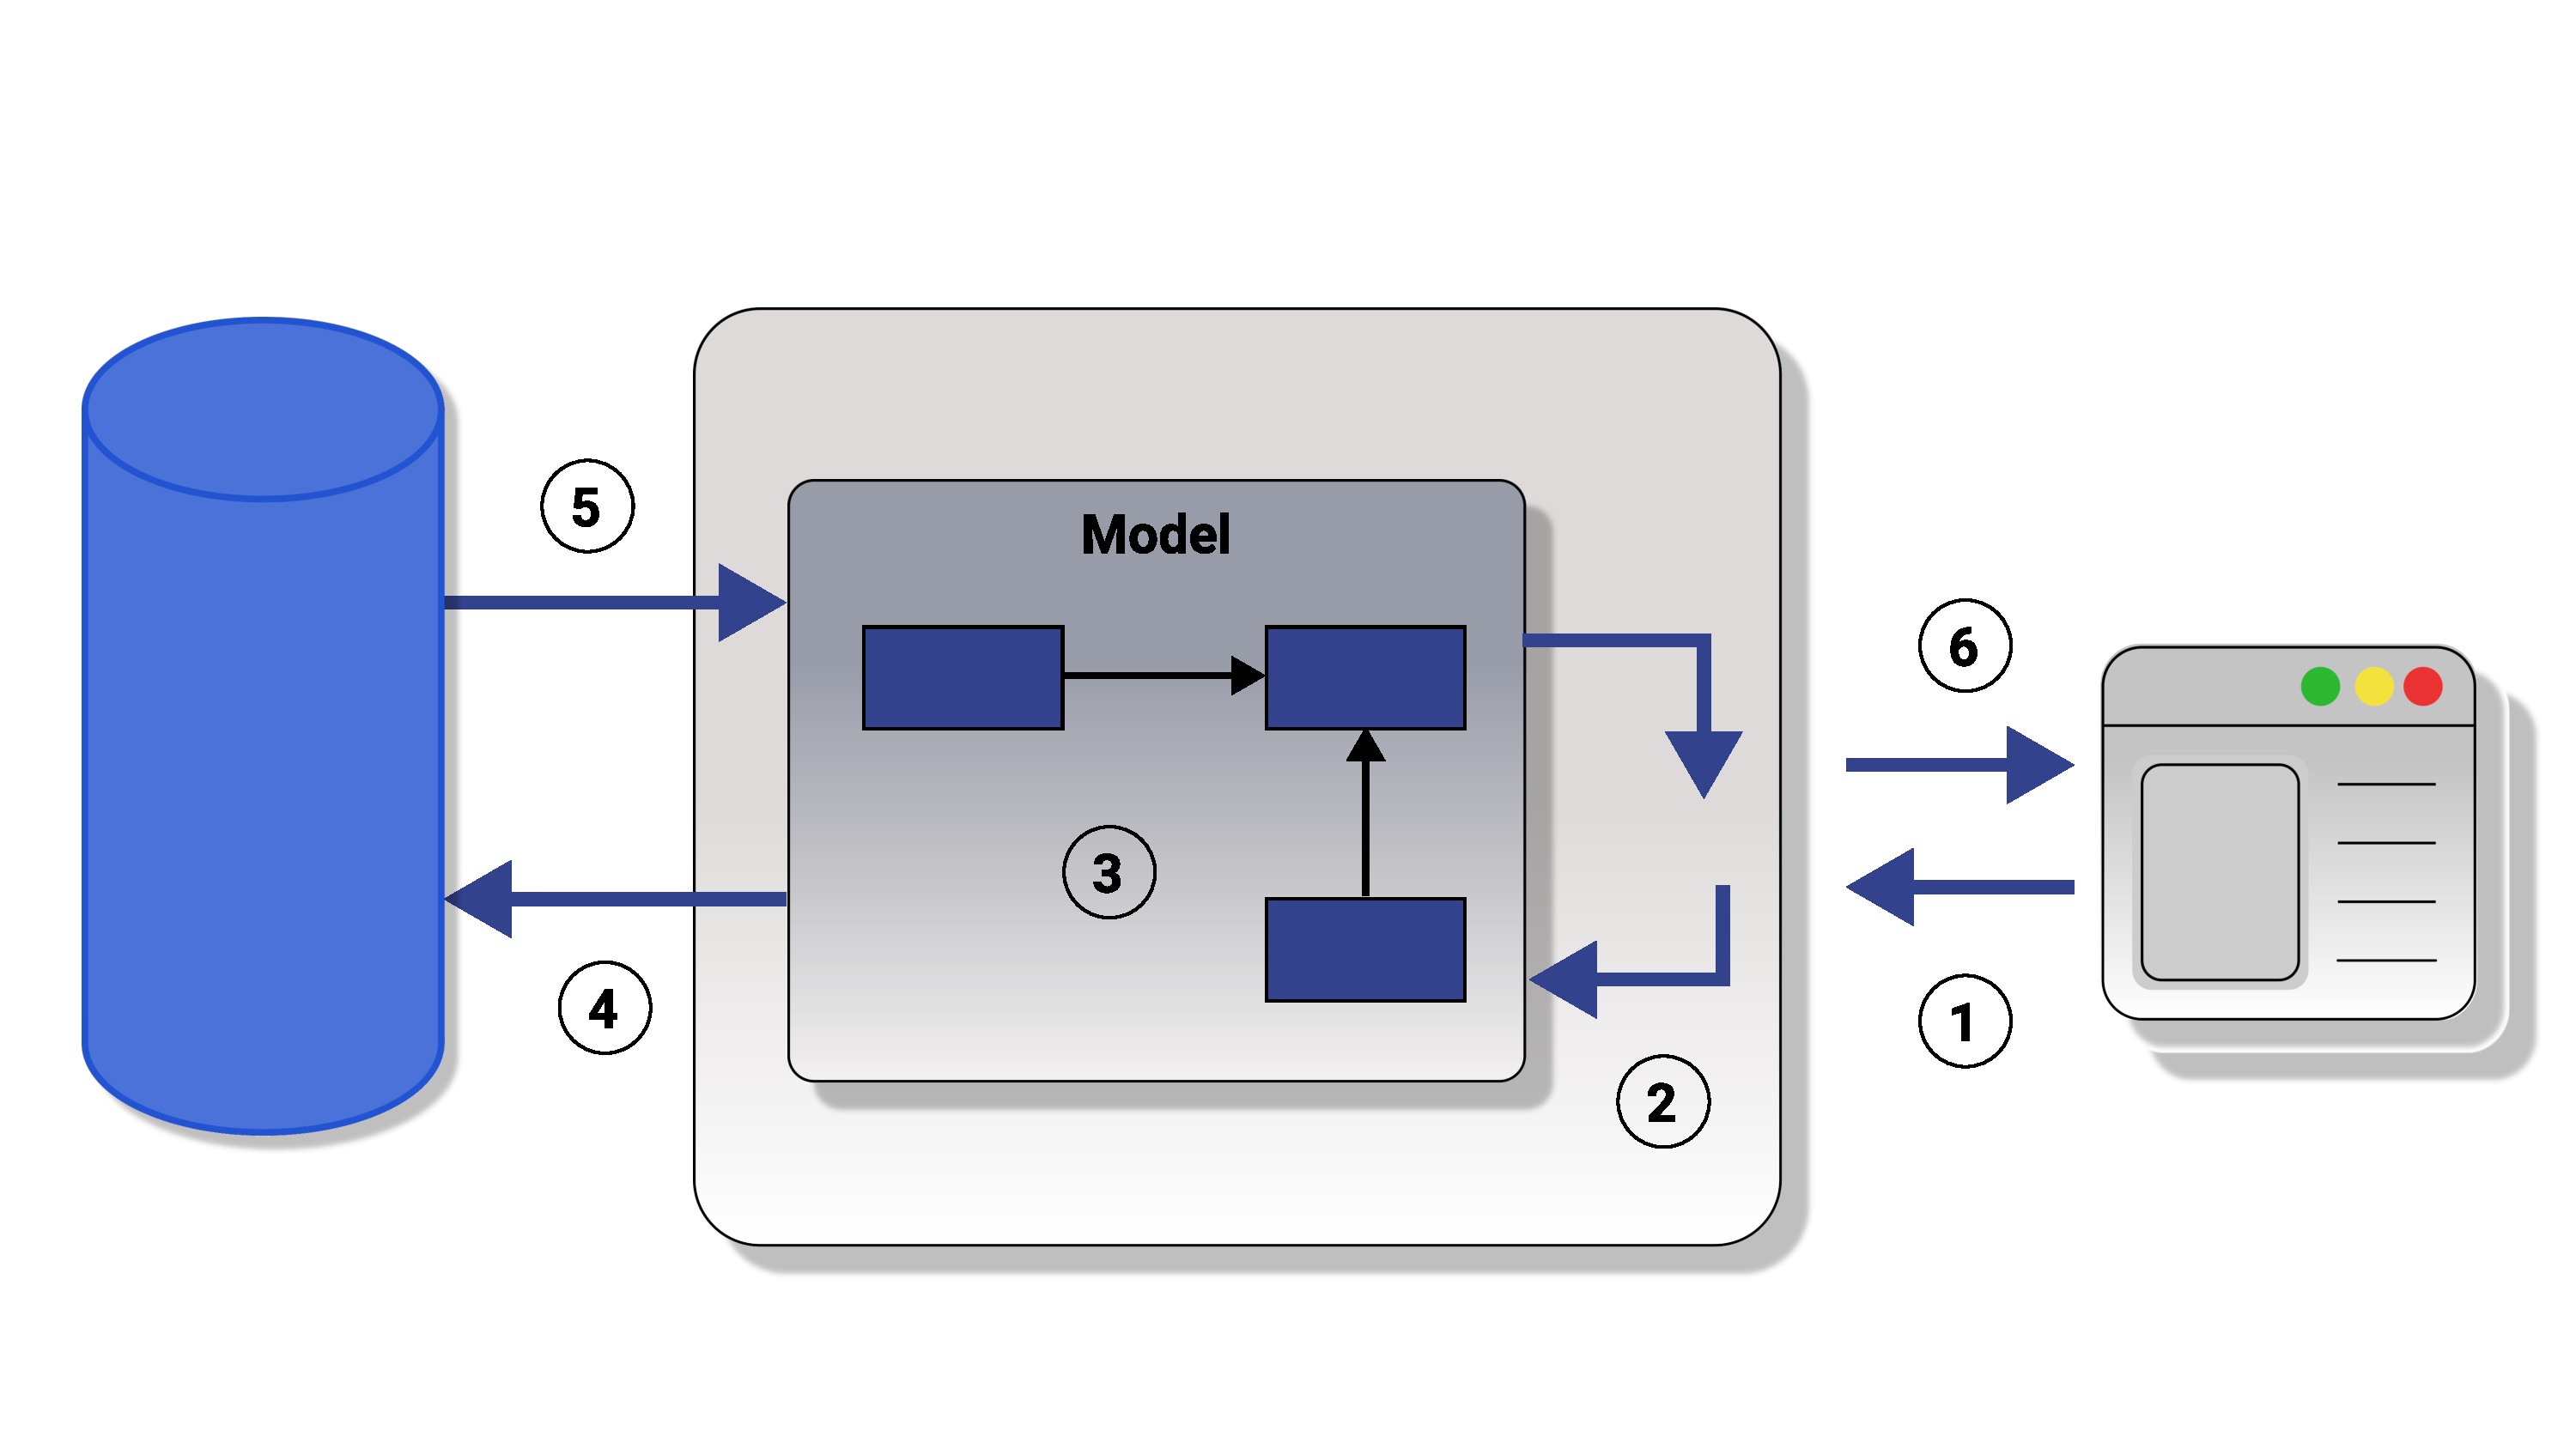
\includegraphics[width=1\textwidth]{Pictures/Services}
    \caption{CQRS Conceptual diagram.
    Source: \href{https://martinfowler.com/bliki/CQRS.html}{Martin Fowler}.}\label{fig:figure9}
\end{figure}
As it stated in previous section, monolithic architecture provides a quite strong coupling between application
components.
Moreover, as monolith grow horizontally, its services layer grows as well.
This process leads to very huge code base which is very difficult to support and extend.
We attach the following
\href{https://github.com/smartstore/SmartStoreNET/blob/4.x/src/Presentation/SmartStore.Web/Controllers/CatalogHelper.cs}
{link}
as an example of such approach.
To avoid the natural results of monolithic architecture, that are huge classes for thousands lines, we have to dive into
design patterns [\cite{rising1998design}].
Precisely, the mediator design pattern would help to decouple the service layer from presentation layer.
Mediator -- is a behavioral design pattern [\cite{rasche2016building}] that lets you reduce chaotic dependencies between objects.
The pattern restricts direct communications between the objects and forces them to collaborate only via a mediator object.
In other words, mediator allows the communication between two entities, such that entities doesn't know each other.
The Mediator pattern suggests that you should cease all direct communication between the components which you want to make
independent of each other.
Instead, these components must collaborate indirectly, by calling a special mediator object that redirects the calls to
appropriate components.
As a result, the components depend only on a single mediator class instead of being coupled to dozens of their colleagues.
In context of .NET platform there are multiple implementation of the Mediator, the most widely known and used is the
\href{https://github.com/jbogard/MediatR}{MediatR}, which we use in our project.
Another, yet popular approach is the CQRS, which stands for Command-Query Responsibility Segregation.
In brief, it stands that read (query) and write (command) requests should be segregated by their responsibilities.
The CQRS approach in couple with Mediator greatly helps to solve the coupling problem of the monolith architecture.
So what is CQRS precisely?
According to \href{https://martinfowler.com/bliki/CQRS.html}{Martin Fowler},
it is a pattern that first described by Greg Young [\cite{young2010cqrs}].
At its heart is the notion that you can use a different model to update information than the model you use to read information.
For some situations, this separation can be valuable, but beware that for most systems CQRS adds risky complexity.
The mainstream approach people use for interacting with an information system is to treat it as a CRUD datastore.
By this meant that we have mental model of some record structure where we can create new records, read records,
update existing records, and delete records when we're done with them.
In the simplest case, our interactions are all about storing and retrieving these records.
As our needs become more sophisticated we steadily move away from that model.
We may want to look at the information in a different way to the record store, perhaps collapsing multiple records into one,
or forming virtual records by combining information for different places.
On the update side we may find validation rules that only allow certain combinations of data to be stored, or may even infer
data to be stored that's different from that we provide.
For instance, the idea of command-query segregation is displayed at the following image

\begin{figure}[H]
    \centering
    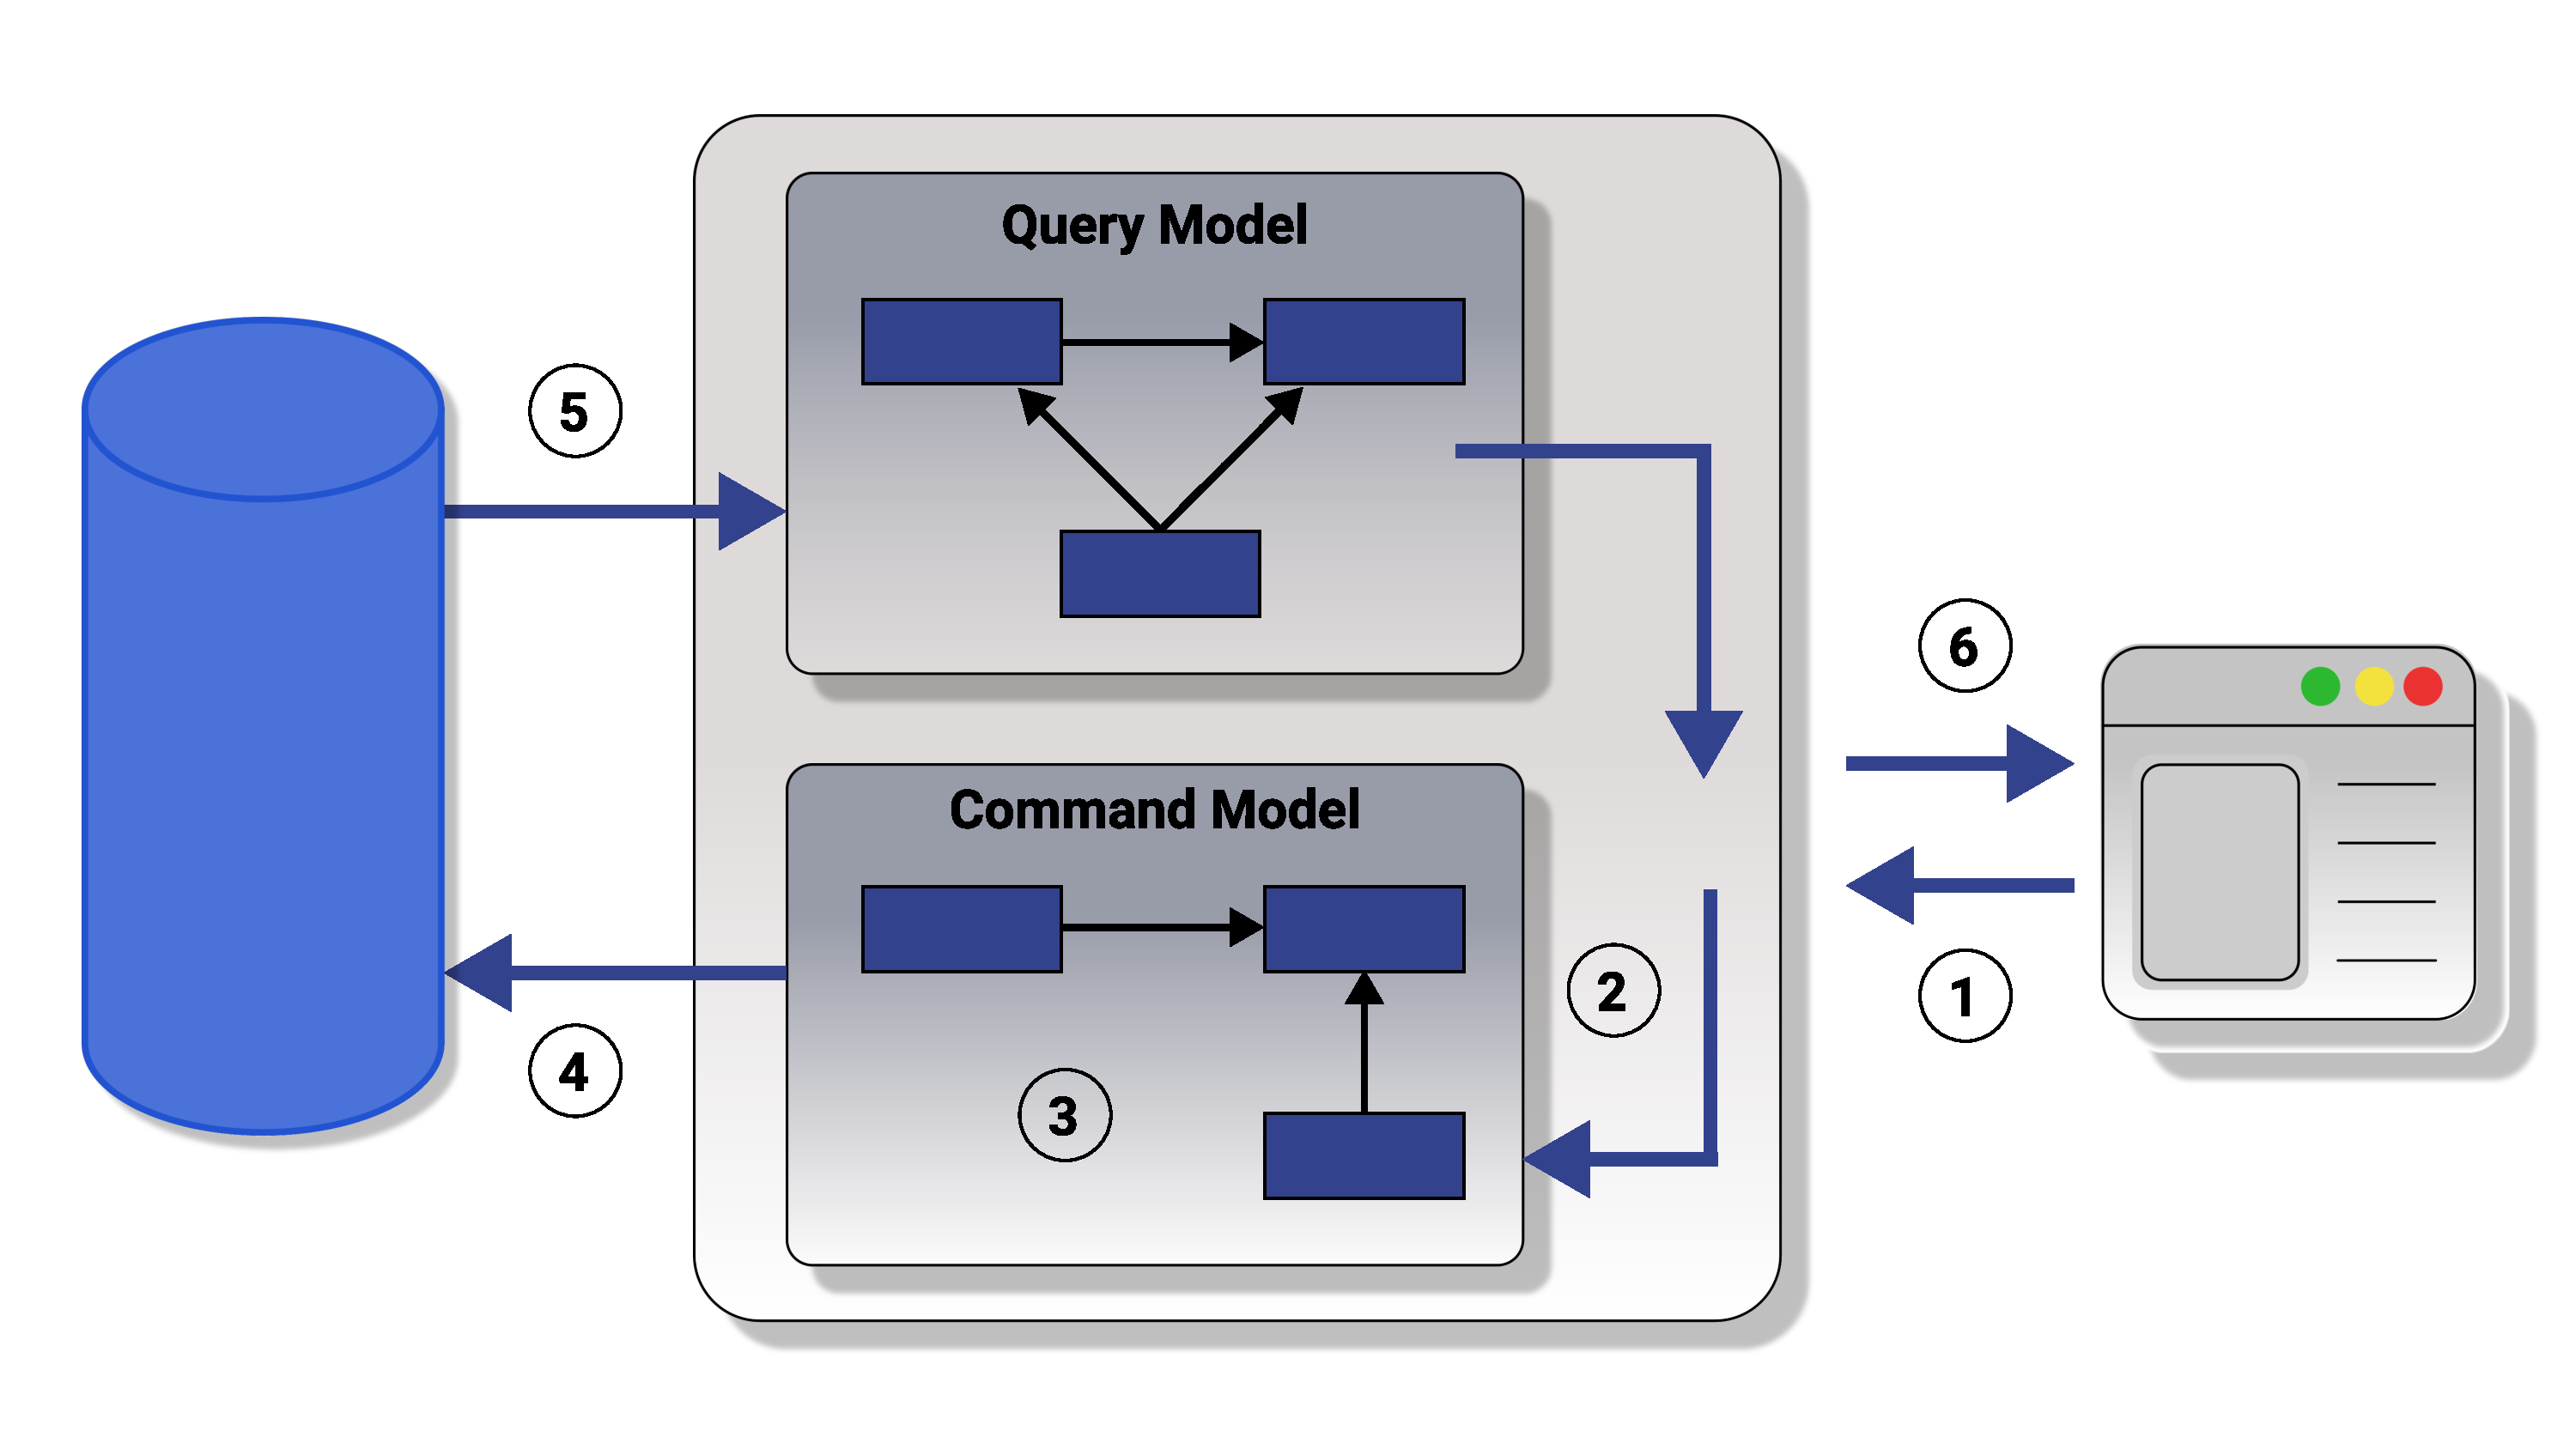
\includegraphics[width=1\textwidth]{Pictures/cqrs.pdf}
    \caption{CQRS Conceptual diagram.
    Source: \href{https://martinfowler.com/bliki/CQRS.html}{Martin Fowler}.}
    \label{fig:figure}
\end{figure}

\begin{enumerate}
    \item User makes a change in UI\@.
    \item Application routes information to command model.
    \item Command model executes validation and business logic.
    \item Command model updates the database.
    \item Query model reads from database.
    \item Query service update presentation from query model.
\end{enumerate}

Despite these benefits, you should be very cautious about using CQRS\@.
Many information systems fit well with the notion of an information base that is updated in the same way that it's read,
adding CQRS to such a system can add significant complexity.
I've certainly seen cases where it's made a significant drag on productivity, adding an unwarranted amount of risk to the
project, even in the hands of a capable team.
So while CQRS is a pattern that's good to have in the toolbox, beware that it is difficult to use well and you can easily
chop off important bits if you mishandle it.

As a short conclusion, we may state that CQRS and Mediator pattern will not entirely solve the coupling problems the monolith,
however will make project much more simplistic and intuitively understood.
It is worth to keep is simple,
even relatively simple project may grow to the sizes of universe without proper architectural solutions.

Over whole data entities, we prefer to use universally unique identifier (UUID) or namely globally unique identifier (GUID),
a 128-bit label used for information in computer systems [\cite{leach2005universally}].
Simply, because it does not force us to keep a sequence on database side.
Sequence -- is a special entity provided in PostgreSQL relational databases.
It is responsible for generating unique values and sometimes causes a problems during migration of the database.
But still, are GUID identifiers are really always unique?
Well, each generated GUID is not guaranteed to be unique, the total number of unique keys $2^{128}$ or $3.4 \times 10^{38}$
is so large that the probability of the same number being generated twice is very small.
For example, consider the observable universe, which contains about $5 \times 10^{22}$ stars.
Every star could then have $6.8 \times 10^{15}$ universally unique GUIDs.
If you are scared of the same GUID values then put two of them next to each other.
If you are too paranoid then put three [\cite{GUIDSo}].